\documentclass[tikz]{standalone}
\usepackage{amsmath,amssymb}
\usepackage{pgfplots,multicol}

\pgfplotsset{compat=1.10}
\usepgfplotslibrary{fillbetween}

\begin{document}



 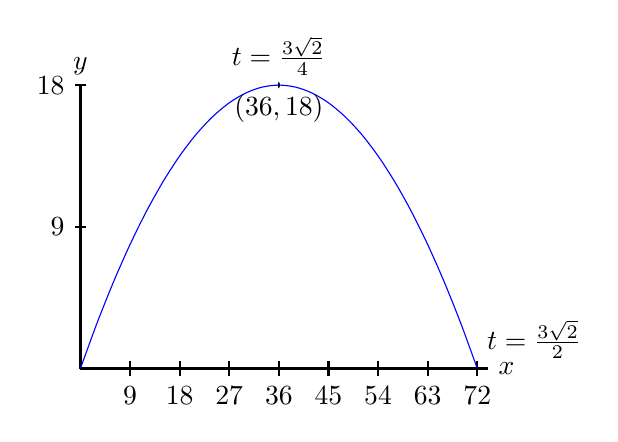
\begin{tikzpicture}[xscale=0.07,yscale=0.2]
        \draw[-,thick] (0,0) -- (74,0) node[right] {$x$};
         \draw[-,thick] (0,0) -- (0,18) node[above] {$y$};

	\foreach \x in {9,18,...,72}
	 \draw[-,thick] (\x,0.5) -- (\x,-0.5) node[below] {\x};
	 
	 	\foreach \y in {9,18}
	 \draw[-,thick] (1,\y) -- (-1,\y) node[left] {\y};
	
	\draw[-,smooth,domain=0:72,blue] plot(\x,{-\x*\x/72+\x});
	

	\draw[fill=black] (72,0) circle (0.1cm) node[above right] {$t=\frac{3\sqrt{2}}{2}$};
	\draw[fill=black] (36,18) circle (0.1cm) node[below] {$(36,18)$};
		\draw[fill=black] (36,18) circle (0.1cm) node[above] {$t=\frac{3\sqrt{2}}{4}$};
	

\end{tikzpicture}


	
\end{document}
